\documentclass[12pt]{article}
\usepackage{array}
\usepackage{amsmath}
\usepackage{mathtools}
\usepackage{textcomp, gensymb}
\usepackage{graphicx}
\usepackage{float}
\usepackage{caption}

\allowdisplaybreaks

\begin{document}

    \title{Time Constants for an RC Circuit and an LR Circuit}
    \author{Ryan Coyne}
    \maketitle

    \section{Abstract/Procedure/Conclusion}
        In this lab, we measured the time constants, \(\tau\), for three RC and three LR circuits. Each RC circuit was set up as in Figure 1. The first had a resistor with a resistance of 100 \(\Omega\) and a capacitor with a capacitance of 330 \(\mu\)F. The second had a resistor with a resistance of 10 \(\Omega\) and a capacitor with a capacitance of 100 \(\mu\)F. The first had a resistor with a resistance of 10 \(\Omega\) and a capacitor with a capacitance of 100 \(\mu\)F. The LR circuits were set up as shown in Figure 2. They all used the same inductor with an inductance of 8.2 mH and a resistance of 6.5 \(\Omega\). The first had a resistor with a resistance of 10 \(\Omega\). The second had a resistor with a resistance of 33 \(\Omega\). The third had a resistor with a resistance of 100 \(\Omega\). The power source was a signal generator set to create a square wave with a frequency around 1 kHz and an amplitude of 5 V.
    \begin{figure}[H]
        \centering
        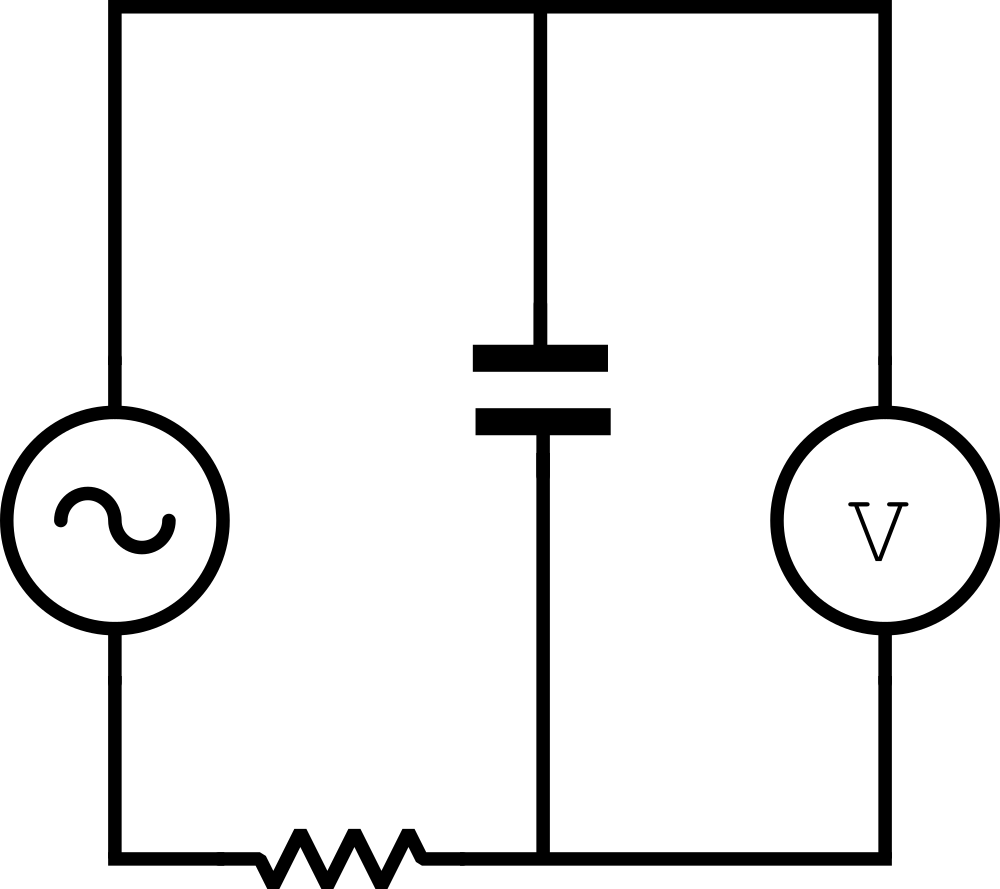
\includegraphics{RCSetup.png}
        \caption{RC circuit: Experimental setup}
    \end{figure}

    \begin{figure}[H]
        \centering
        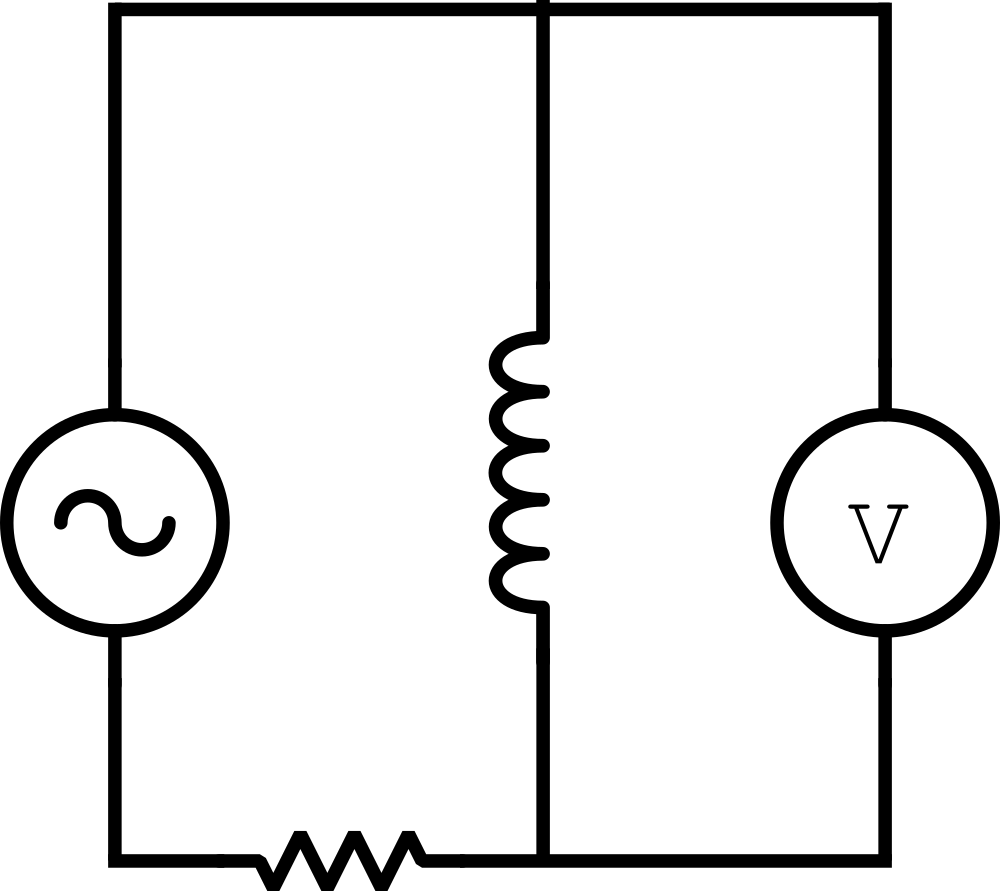
\includegraphics{LRSetup.png}
        \caption{LR circuit: Experimental setup}
    \end{figure}

    \section{Data}
        \begin{table}[H]
            \centering
            \begin{tabular}{c|c|c|c|c}
                &\(C\ (\mathrm{\mu F})\) & \(R\ (\Omega)\) & \(\tau\) (s) & \(\tau_{meas}\) (s)\\
                \hline
                1&330 & 100 & 0.033 & 0.036 \\
                2&100 & 10 & 0.0010 & 0.0011\\
                3&100 & 33 & 0.0033 & 0.0036 \\
            \end{tabular}
            \caption{RC circuit: Capacitance and resistance.}
        \end{table}
        \begin{table}[H]
            \centering
            \begin{tabular}{c|c|c|c|c}
                &\(L\) (H) & \(R\ (\Omega)\) & \(\tau\) (s)& \(\tau_{meas}\) (s)\\
                \hline
                1&0.0082 & 16.5 & 0.000497 & 0.000078\\
                2&0.0082 & 39.5 & 0.00021 & 0.00021\\
                3&0.0082 & 106.5 & 0.000077 & 0.00051
            \end{tabular}
            \caption{LR circuit: Inductance and resistance.}
        \end{table}
        \begin{figure}[H]
            \centering
            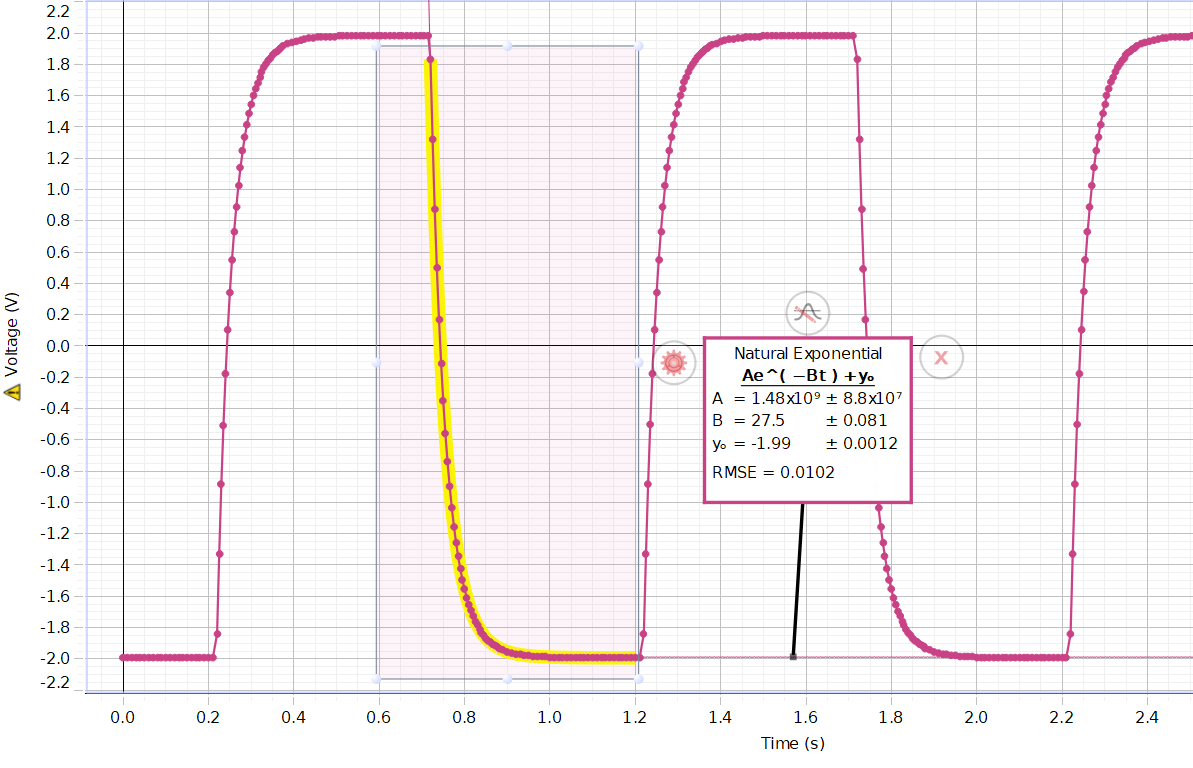
\includegraphics[width=0.75\linewidth]{RC1.png}
            \caption{RC circuit 1 plot.}
        \end{figure}
        \begin{figure}[H]
            \centering
            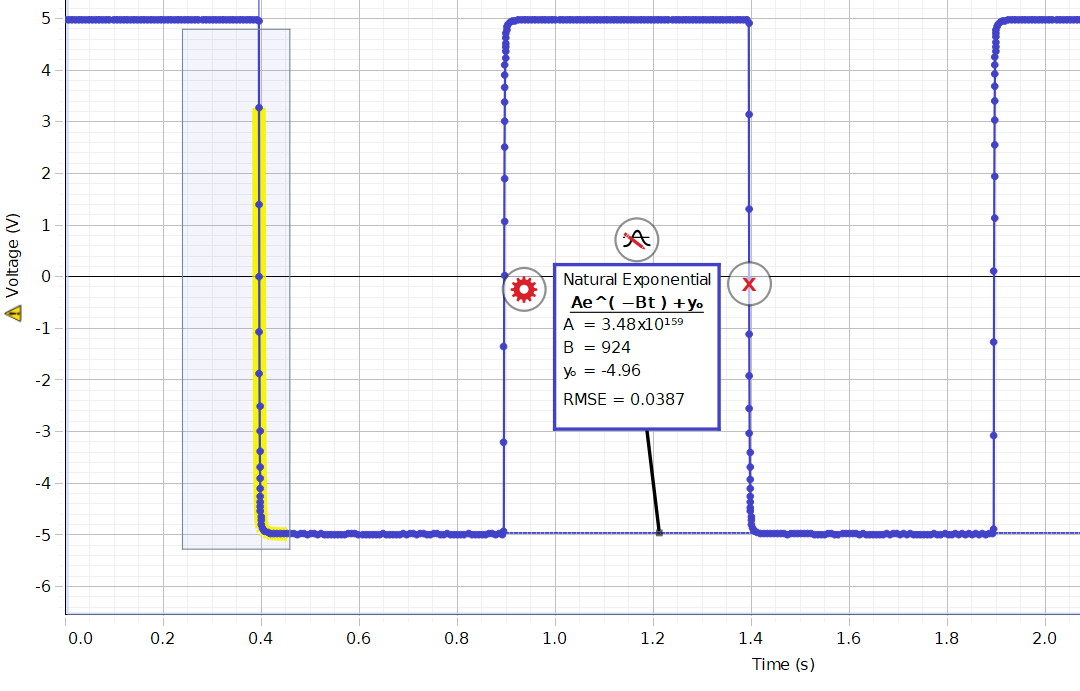
\includegraphics[width=0.75\linewidth]{RC2.png}
            \caption{RC circuit 2 plot.}
        \end{figure}
        \begin{figure}[H]
            \centering
            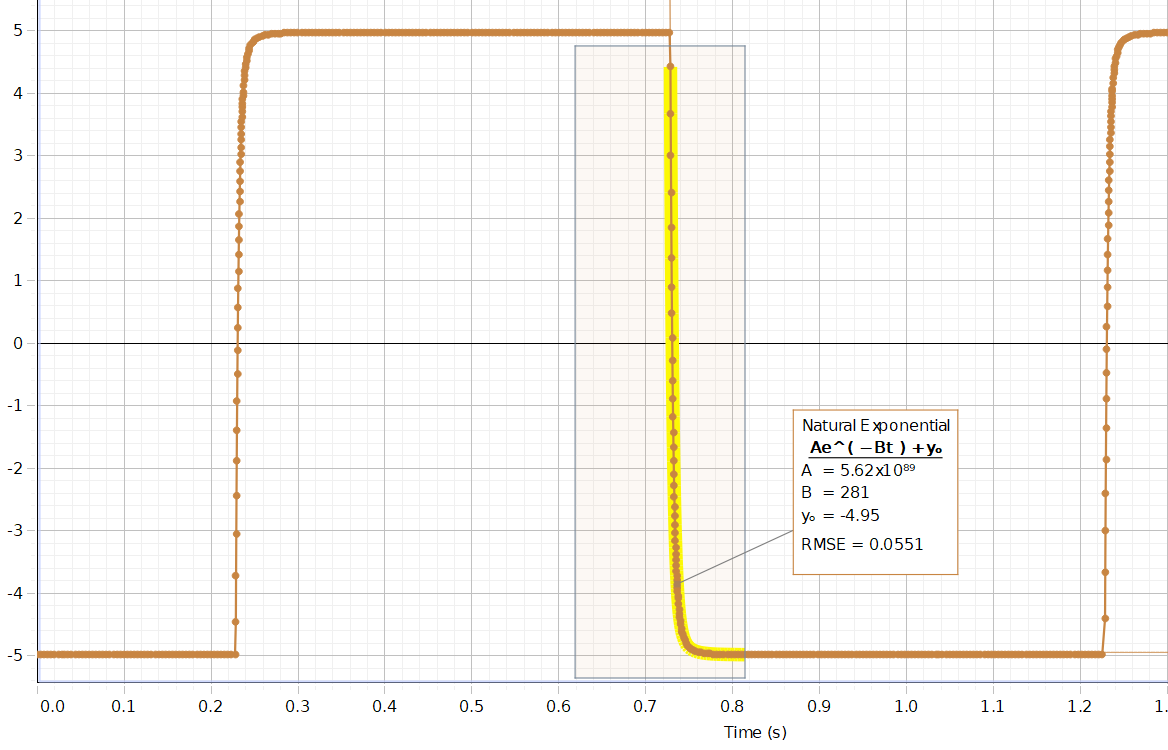
\includegraphics[width=0.75\linewidth]{RC3.png}
            \caption{RC circuit 3 plot.}
        \end{figure}
        \begin{figure}[H]
            \centering
            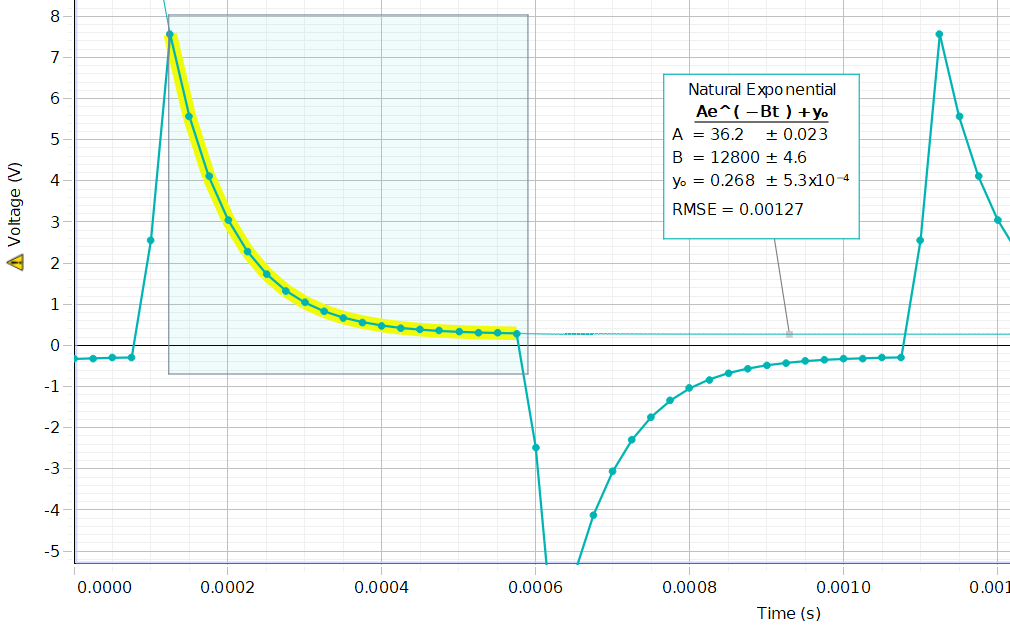
\includegraphics[width=0.75\linewidth]{LR1.png}
            \caption{LR circuit 1 plot.}
        \end{figure}
        \begin{figure}[H]
            \centering
            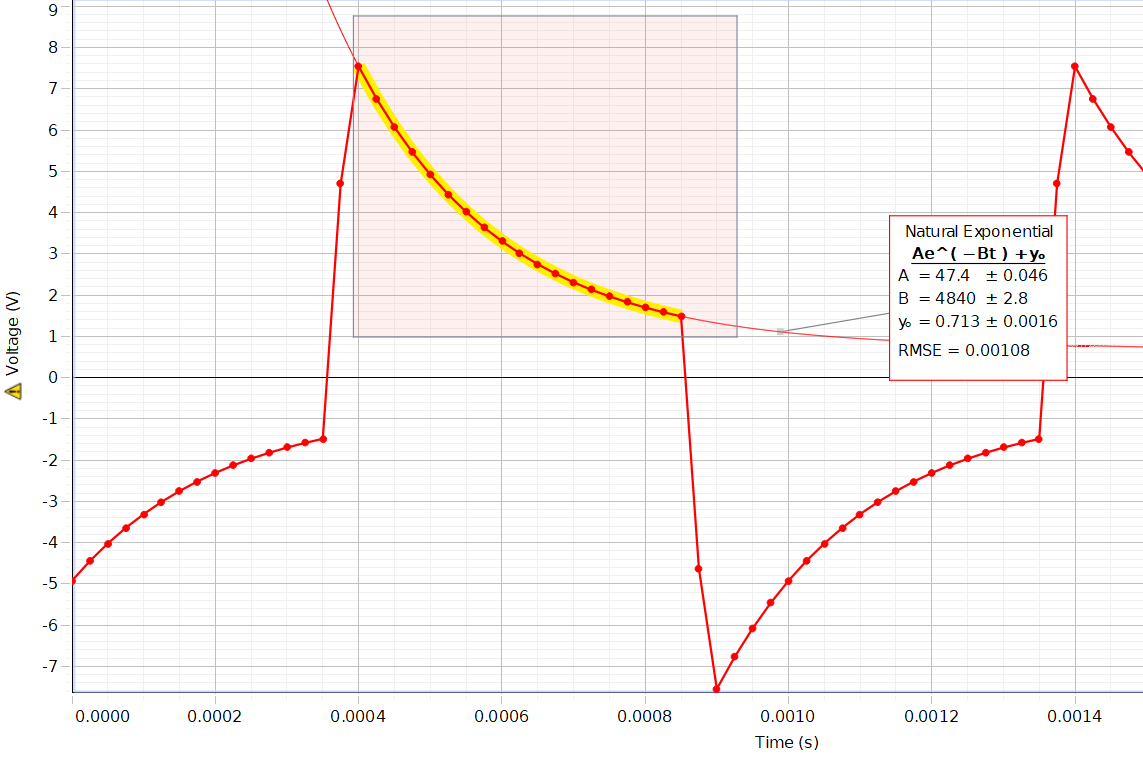
\includegraphics[width=0.75\linewidth]{LR2.png}
            \caption{LR circuit 2 plot.}
        \end{figure}
        \begin{figure}[H]
            \centering
            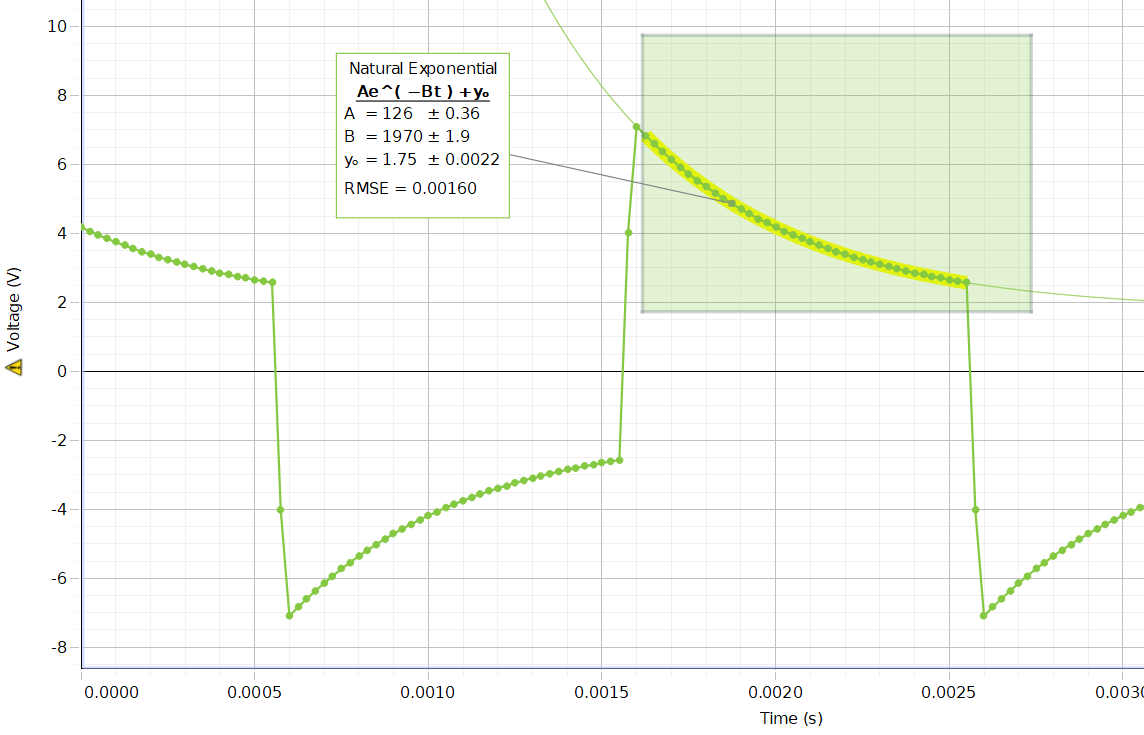
\includegraphics[width=0.75\linewidth]{LR3.png}
            \caption{LR circuit 3 plot.}
        \end{figure}
    \section{Calculations}
        \begin{alignat*}{3}
            (1)\ \ &&
            Q&=C\Delta V_c\\
            (2)\ \ 
            &&\sigma_{R_1} & = 5\mathrm{\ \Omega}\\
            &&\sigma_{R_2} & = 1.65\mathrm{\ \Omega}\\
            &&\sigma_{R_3} & = 0.5\mathrm{\ \Omega}\\
            &&\frac{\sigma_{R_1}}{R_1} & = \frac{5 \mathrm{\ \Omega}}{100 \mathrm{\ \Omega}}\\
            &&\frac{\sigma_{R_2}}{R_2} & = \frac{1.65 \mathrm{\ \Omega}}{33 \mathrm{\ \Omega}}\\
            &&\frac{\sigma_{R_3}}{R_3} & = \frac{0.5 \mathrm{\ \Omega}}{10 \mathrm{\ \Omega}}\\
            &&\frac{\sigma_{R_1}}{R_1} & = \frac{\sigma_{R_2}}{R_2} = \frac{\sigma_{R_3}}{R_3}\\
            &&&=5\%\\
            &&\sigma_{C_1} &= 66\ \mathrm{\mu F}\\
            &&\sigma_{C_2} &= 20\ \mathrm{\mu F}\\
            &&\frac{\sigma_{C_1}}{C_1} &= \frac{66\ \mathrm{\mu F}}{330\ \mathrm{\mu F}}\\
            &&\frac{\sigma_{C_2}}{C_2} &= \frac{20\ \mathrm{\mu F}}{100\ \mathrm{\mu F}}\\
            &&\frac{\sigma_{C_1}}{C_1} &=\frac{\sigma_{C_2}}{C_2}\\
            &&& = 20\%\\
            (3)\ \
            &&\overline{\tau_1} &= 330 \ \mathrm{\mu F} \cdot 100 \ \mathrm{\Omega}\\
            &&&=0.033\text{ s}\\
            &&\tau_{1,R} &= 330 \ \mathrm{\mu F} \cdot (100+5) \ \mathrm{\Omega}\\
            &&& = 0.03465\ \mathrm{s}\\
            &&\tau_{1,C} &= (330+66)\ \mathrm{\mu F} \cdot 100 \ \mathrm{\Omega}\\
            &&&=0.0396\\
            &&\sigma_{\tau_1} &= 0.0068\ \text{s}\\
            (4)\ \
            &&\sigma_{R_4} & = 0.825\mathrm{\ \Omega}\\
            &&\sigma_{R_5} & = 1.975\mathrm{\ \Omega}\\
            &&\sigma_{R_6} & = 5.325\mathrm{\ \Omega}\\
            &&\frac{\sigma_{R_4}}{R_4} & = \frac{0.825 \mathrm{\ \Omega}}{16.5 \mathrm{\ \Omega}}\\
            &&\frac{\sigma_{R_5}}{R_5} & = \frac{1.975 \mathrm{\ \Omega}}{39.5 \mathrm{\ \Omega}}\\
            &&\frac{\sigma_{R_6}}{R_6} & = \frac{5.325 \mathrm{\ \Omega}}{106.5 \mathrm{\ \Omega}}\\
            &&\frac{\sigma_{R_4}}{R_4} & = \frac{\sigma_{R_5}}{R_5} = \frac{\sigma_{R_6}}{R_6}\\
            &&&=5\%\\
            (5)\ \ 
            &&\overline{\tau_4} &= \frac{0.0082 \text{ H}}{16.5 \Omega}\\
            &&&= 0.000497 \text{ s}\\
            &&\tau_{4,R} &= \frac{0.0082 \text{ H}}{(16.5 + 0.825) \Omega}\\
            &&&= 0.000473 \text{ s}\\
            &&\sigma_{\tau_4} &= \overline{\tau_4} - \tau_{4,R}\\
            &&& = 0.000497 \text{ s} - 0.000473 \text{ s}\\
            &&& = 0.000024 \text{ s}
        \end{alignat*}
\end{document}